% !TEX TS-program = xelatex
\documentclass[11pt,landscape,a4paper]{article}
\usepackage[normalem]{ulem}
\usepackage{amsmath}
\usepackage{graphicx}
\usepackage{outlines}
\graphicspath{{./}}
\usepackage{tikz}
\usetikzlibrary{shapes,positioning,arrows,fit,calc,graphs,graphs.standard}
\usepackage[nosf]{kpfonts}
\usepackage[t1]{sourcesanspro}
\usepackage{multicol}
\usepackage{wrapfig}
\usepackage[top=0mm,bottom=1mm,left=0mm,right=1mm]{geometry}
\usepackage[framemethod=tikz]{mdframed}
\usepackage{microtype}
\usepackage{tabularx}
\usepackage{hhline}
\usepackage{makecell}
\usepackage{mathtools}
\usepackage{listings}

\DeclarePairedDelimiter{\ceil}{\lceil}{\rceil}

\newcommand\codeblue[1]{\textcolor{blue}{\code{#1}}}

\usepackage{lastpage}
\usepackage{datetime}
\yyyymmdddate
\renewcommand{\dateseparator}{-}
\let\bar\overline

\definecolor{myblue}{cmyk}{1,.72,0,.38}

\def\firstcircle{(0,0) circle (1.5cm)}
\def\secondcircle{(0:2cm) circle (1.5cm)}

\colorlet{circle edge}{myblue}
\colorlet{circle area}{myblue!5}

\tikzset{filled/.style={fill=circle area, draw=circle edge, thick},
outline/.style={draw=circle edge, thick}}

\pgfdeclarelayer{background}
\pgfsetlayers{background,main}

%\everymath\expandafter{\the\everymath \color{myblue}}
%\everydisplay\expandafter{\the\everydisplay \color{myblue}}


\renewcommand{\baselinestretch}{.8}
\pagestyle{empty}

\global\mdfdefinestyle{header}{%
  linecolor=gray,linewidth=1pt,%
  leftmargin=0mm,rightmargin=0mm,skipbelow=0mm,skipabove=0mm,
}

\newcommand{\header}{
  \begin{mdframed}[style=header]
    \footnotesize
    \sffamily
    CS2102 Midterm Cheatsheet v1.0 (\today)\\
    by~Aadit Rahul Kamat,~page~\thepage~of~\pageref{LastPage}
  \end{mdframed}
}

\let\counterwithout\relax
\let\counterwithin\relax
\usepackage{chngcntr}

\usepackage{verbatim}

\usepackage{etoolbox}
\makeatletter
\preto{\@verbatim}{\topsep=0pt \partopsep=0pt }
\makeatother

\counterwithin*{equation}{section}
\counterwithin*{equation}{subsection}
\usepackage{enumitem}
\newlist{legal}{enumerate}{10}
\setlist[legal]{label*=\arabic*.,leftmargin=2.5mm}
\setlist[itemize]{leftmargin=3mm}
\setlist[enumerate]{leftmargin=3.5mm}
\setlist{nosep}
\usepackage{minted}

\def\code#1{\texttt{#1}}

\newenvironment{descitemize} % a mixture of description and itemize
{\begin{description}[leftmargin=*,before=\let\makelabel\descitemlabel]}
{\end{description}}

\newcommand{\descitemlabel}[1]{%
  \textbullet\ \textbf{#1}%
}
\makeatletter



\renewcommand{\section}{\@startsection{section}{1}{0mm}%
  {.2ex}%
  {.2ex}%x
{\color{myblue}\sffamily\small\bfseries}}
\renewcommand{\subsection}{\@startsection{subsection}{1}{0mm}%
  {.2ex}%
  {.2ex}%x
{\sffamily\bfseries}}
\renewcommand{\subsubsection}{\@startsection{subsubsection}{1}{0mm}%
  {.2ex}%
  {.2ex}%x
{\rmfamily\bfseries}}



\def\multi@column@out{%
  \ifnum\outputpenalty <-\@M
    \speci@ls \else
  \ifvoid\colbreak@box\else
    \mult@info\@ne{Re-adding forced
    break(s) for splitting}%
    \setbox\@cclv\vbox{%
      \unvbox\colbreak@box
    \penalty-\@Mv\unvbox\@cclv}%
  \fi
  \splittopskip\topskip
  \splitmaxdepth\maxdepth
  \dimen@\@colroom
  \divide\skip\footins\col@number
  \ifvoid\footins \else
    \leave@mult@footins
  \fi
  \let\ifshr@kingsaved\ifshr@king
    \ifvbox \@kludgeins
      \advance \dimen@ -\ht\@kludgeins
      \ifdim \wd\@kludgeins>\z@
        \shr@nkingtrue
      \fi
    \fi
    \process@cols\mult@gfirstbox{%
      %%%%% START CHANGE
      \ifnum\count@=\numexpr\mult@rightbox+2\relax
        \setbox\count@\vsplit\@cclv to \dimexpr \dimen@-1cm\relax
        \setbox\count@\vbox to \dimen@{\vbox to 1cm{\header}\unvbox\count@\vss}%
      \else
        \setbox\count@\vsplit\@cclv to \dimen@
      \fi
      %%%%% END CHANGE
      \set@keptmarks
      \setbox\count@
      \vbox to\dimen@
      {\unvbox\count@
        \remove@discardable@items
    \ifshr@nking\vfill\fi}%
    }%
    \setbox\mult@rightbox
    \vsplit\@cclv to\dimen@
    \set@keptmarks
    \setbox\mult@rightbox\vbox to\dimen@
    {\unvbox\mult@rightbox
      \remove@discardable@items
  \ifshr@nking\vfill\fi}%
    \let\ifshr@king\ifshr@kingsaved
  \ifvoid\@cclv \else
    \unvbox\@cclv
    \ifnum\outputpenalty=\@M
  \else
    \penalty\outputpenalty
  \fi
  \ifvoid\footins\else
    \PackageWarning{multicol}%
    {I moved some lines to
      the next page.\MessageBreak
      Footnotes on page
    \thepage\space might be wrong}%
  \fi
  \ifnum \c@tracingmulticols>\thr@@
\hrule\allowbreak \fi
  \fi
  \ifx\@empty\kept@firstmark
    \let\firstmark\kept@topmark
    \let\botmark\kept@topmark
  \else
    \let\firstmark\kept@firstmark
    \let\botmark\kept@botmark
  \fi
  \let\topmark\kept@topmark
  \mult@info\tw@
  {Use kept top mark:\MessageBreak
    \meaning\kept@topmark
    \MessageBreak
    Use kept first mark:\MessageBreak
    \meaning\kept@firstmark
    \MessageBreak
    Use kept bot mark:\MessageBreak
    \meaning\kept@botmark
    \MessageBreak
    Produce first mark:\MessageBreak
    \meaning\firstmark
    \MessageBreak
    Produce bot mark:\MessageBreak
    \meaning\botmark
  \@gobbletwo}%
  \setbox\@cclv\vbox{\unvbox\partial@page
  \page@sofar}%
  \@makecol\@outputpage
  \global\let\kept@topmark\botmark
  \global\let\kept@firstmark\@empty
  \global\let\kept@botmark\@empty
  \mult@info\tw@
  {(Re)Init top mark:\MessageBreak
    \meaning\kept@topmark
  \@gobbletwo}%
  \global\@colroom\@colht
  \global \@mparbottom \z@
  \process@deferreds
\@whilesw\if@fcolmade\fi{\@outputpage
    \global\@colroom\@colht
  \process@deferreds}%
  \mult@info\@ne
  {Colroom:\MessageBreak
    \the\@colht\space
    after float space removed
  = \the\@colroom \@gobble}%
  \set@mult@vsize \global
  \fi}
  \global\let\tikz@ensure@dollar@catcode=\relax

  \def\mathcolor#1#{\@mathcolor{#1}}
  \def\@mathcolor#1#2#3{%
    \protect\leavevmode
    \begingroup
    \color#1{#2}#3%
    \endgroup
  }

  \makeatother
  \setlength{\parindent}{0pt}

  \setminted{tabsize=2, breaklines}
  % Remove belowskip of minted
  \setlength\partopsep{-\topsep}


  \newcolumntype{a}{>{\hsize=1.5\hsize}X}
%   \newcolumntype{b}{>{\hsize=.25\hsize}X}

  \setlength\columnsep{1.5pt}
  \setlength\columnseprule{0.1pt}

\begin{document}
\setlength{\abovedisplayskip}{0pt}
\setlength{\belowdisplayskip}{0pt}


\tiny
\begin{multicols*}{4}
  \raggedcolumns
  
  \section{Relational Algebra}
  \begin{outline}
  \1 Superkey: combo of attributes that uniquely defines its tuples
  \1 Key (e.g candidate key, foreign key) : A type of superkey that is minimal: no proper subset of key is a superkey
  \1 Domain: a set of atomic values
    \2 Each value of an attribute $A_i$ is either domain($A_i$) or null
  \1 Foreign key constraint: each foreign key value in referencing relation must either:
    \2 appear as primary key value in referenced relation

        or

    \2 be a null value
 \1 Set operators require input relations to be union compatible i.e. two relations that:
    \2 have the same number of attributes
    \2 the corresponding attributes have the same domains

  \1 Union compatible relations do not necessarily use the same attribute names

  \1 Cross product:

    $$R \times S = {(a, b, c, x, y) | (a, b, c) ∈ R, (x, y) ∈ S}$$

  \1 Join: Combines cross product and selection (and possibly projection)
    \2 Inner:

    $$R ⊲⊳_c S = σ_c(R \times S)$$

    \2 Natural: Inner join based on renamed attributes

        $$R ⊲⊳_c S = π_ℓ(R ⊲⊳_c ρ_{a_1:b_1},... ,_{a_n:b_n}(S))$$

     \2 A \textbf{dangling tuple} is a tuple in a join operand that does not participate in the join
    \1 Outer:
        \2 Left:

        $$R →_c S = (R ⊲⊳_c S) ∪ (dangle(R ⊲⊳c S) \times null(S))$$

        \2 Right:

        $$R ←_c S = (R ⊲⊳_c S) ∪ ({null(R)} \times dangle(S ⊲⊳_c R))$$

        \2 Full:

        $$R ↔_c S = (R →_c S) ∪ ({null(R)} \times (S ⊲⊳_c R))$$
  \end{outline}
  \section{ER diagrams}
  \begin{outline}
  \1  Relationship roles are shown explicitly when one entity set appears two or more times in a relationship set

$$Key(R) = A′ \cup \ \bigcup_{E_i \in E′} Key(E_i)$$

\1 Participation constraints:

    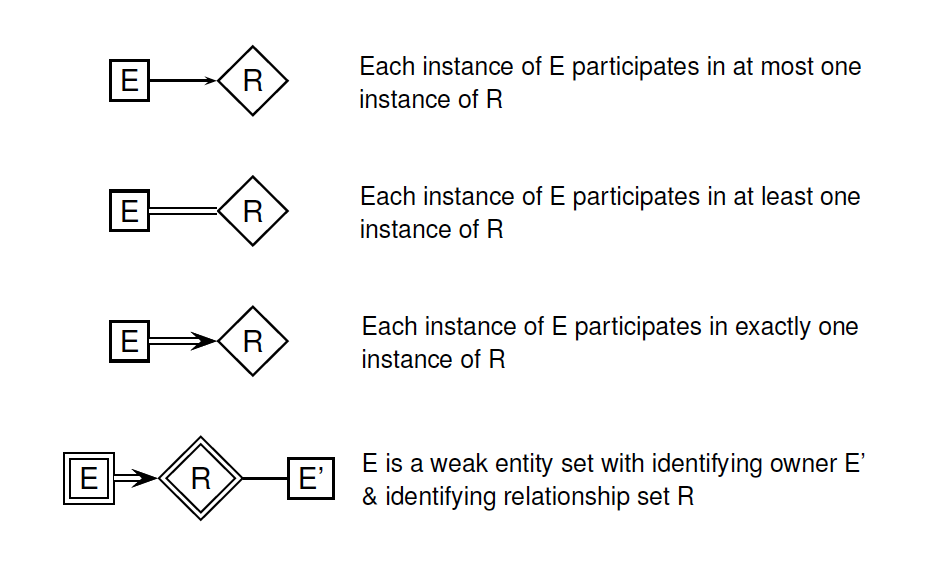
\includegraphics[width=0.8\columnwidth]{CS2102/participation_constraints.png}
\end{outline}
  
\section{SQL}
\begin{outline} 
\1 Comments:  - - or /* */
\1 Commands:
        \2 \textbf{create table}
        \2 \textbf{drop table if exists} <tablename> \textbf{cascade};
        \2 \textbf{insert into} <tablename> values (<values>);
        \2 \textbf{delete from} <tablename> where <condition>;
        \2 \textbf{FOREIGN KEY} ... \textbf{REFERENCES} ... **ON DELETE/UPDATE action**;
        \2 \textbf{alter table} Students \textbf{alter column} dept \textbf{drop default};
        \2 \textbf{alter table} Students \textbf{drop column} dept;
        \2 \textbf{alter table} Students \textbf{add constraint} fk\_grade \textbf{foreign key}
        (grade) \textbf{references} Grades;
\1 Constraint Specifications:
    \2 Column constraints
    \2 Table constraints
    \2 Assertions

\1 Constraint Types:
    \2 Not-null constraints
    \2 Unique constraints
    \2 Primary key constraints
    \2 Foreign key constraints
    \2 Check constraints
    
\1 Constraint violations:
    \2 NO ACTION: rejects delete/update if it violates constraint (default option)
    \2 RESTRICT: similar to NO ACTION except that
        constraint checking can’t be deferred
    \2 CASCADE: propagates delete/update to referencing tuples
    \2 SET DEFAULT: updates foreign keys of referencing tuples to some default value
    \2 SET NULL: updates foreign keys of referencing tuples to null value
    
\1 Transaction:
    begin;
    <SQL Commands>
    commit;

\1 Deferrable constraints:
    \2 deferrable initially deferred
    \2 deferrable initially immediate

        Eg: 
        constraint employees\_fkey foreign key \\ (managerId) references Employees \\
        deferrable initially immediate
\end{outline}

\end{multicols*}
\end{document}
